\section{Proposed Approach: Effective Partnerships Adjustment%
    \footnote{A preliminary version of this approach was presented in \cite{Knight2022smdm}.}}
\label{foi.prop}
Considering the potential drawbacks of pair-based and individual-based models
outlined above in \sref{foi.prior.alt},
an improved approach to modelling HIV transmission via sexual partnerships
within the compartmental framework would be useful.
In this section, I propose such an approach
--- the \emph{Effective Partnerships Adjustment}.
That is, the proposed approach
overcomes the limitations of prior approaches described in \sref{foi.prior.lims},
without the need to change modelling frameworks.
%===================================================================================================
\subsection{Illustrative Scenario}\label{foi.prop.toy}
Consider the moment of one transmission event
in a population of 16 monogamous partnerships, with 25\% infection prevalence
and random mixing by infection status (Figure~\ref{fig:foi.toy.pair}).
Initially, infection prevalence is equal among partners of
susceptible $S$ and infectious $I$ individuals: 6/24 and 2/8, respectively.
Immediately after transmission,
prevalence decreases to 5/23 among partners of $S$ but increases to 4/9 among partners of $I$,
decreasing the population-level transmission risk.
Next, three events are possible:
\begin{enumerate}[label=(\alph*)]
  \item \label{foi.toy.e.t}
  another transmission occurs among the remaining $S$-$I$ partnerships,
  yielding 4/22 prevalence among partners of $S$, and 6/10 among partners of $I$;
  population-level transmission risk decreases further
  \item \label{foi.toy.e.p}
  the partnership from the original transmission ends,
  and both individuals form new partnerships (assumed at random),
  yielding, on average, 9/32 prevalence among partners of both $S$ and $I$;
  population-level transmission risk increases \emph{above} the initial level ($9/32 > 6/24$)
  \item \label{foi.toy.e.q}
  any other partnership ends,
  and both individuals form new partnerships (assumed at random);
  infection prevalence among $S$ and $I$, and population-level transmission risk
  all remain unchanged, on average
\end{enumerate}
Prior compartmental models have effectively assumed that
event \ref{foi.toy.e.p} always occurs before \ref{foi.toy.e.t}
--- \ie the ``instantaneous partnership assumption''.
This assumption is reflected in Figure~\ref{fig:foi.toy.freq},
where the frequentist approximation does not explicitly model any individual partnerships.
This assumption is evidently worse for longer partnerships.
\begin{figure}
  \begin{subfigure}{.5\linewidth}
    \centering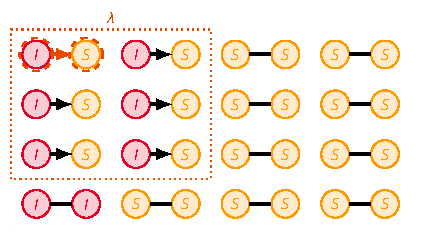
\includegraphics[scale=1]{foi.toy.pair}
    \caption{Pair-wise reality}
    \label{fig:foi.toy.pair}
  \end{subfigure}%
  \begin{subfigure}{.5\linewidth}
    \centering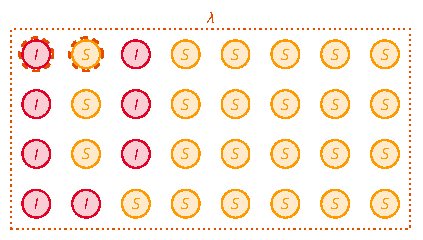
\includegraphics[scale=1]{foi.toy.freq}
    \caption{Frequentist approximation}
    \label{fig:foi.toy.freq}
  \end{subfigure}
  \caption{Comparison of pair-based reality and frequentist approximation
    for a population of 16 pairs with 25\% infection prevalence,
    at the moment of one transmission event}
  \label{fig:foi.toy}
  \floatfoot{
    $S$: susceptible; $I$: infectious; $\lambda$: force of infection;
    dashed circles: individuals involved in transmission event.}
\end{figure}
%===================================================================================================
\subsection{Conceptual Development}\label{foi.prop.concept}
The illustrative scenario highlights how any partnership where transmission has occured
are ``transmission ineffective'' --- \ie seroconcordant ---
and should be removed from the force of infection.
In a compartmental (non-pair-based) model,
these partnerships can be tracked as proportions of individuals: namely,
all individuals who recently acquired infection \emph{and}
all individuals who recently transmitted infection.
Here, I use ``recent'' to mean ``before individuals change partners''.
If some individuals have multiple concurrent partnerships ($K > 1$),
then these individuals should not be removed entirely,
but their numbers of ``effective partnerships'' should be reduced by 1.
If multiple types of partners are considered,
then only the partnership type involved in the transmission should be reduced.
This adjustment to ``effective partnerships'' can then be applied
until these individuals change partners
% TODO: (*) but part of partnership has already passed, so delta_new < delta_total
--- at a rate inversely related to partnership duration: $\delta^{-1}$.
However, during this period, these individuals should still be modelled
to progress as usual through different stages of infection, activity group turnover, etc.
\par
Using this conceptual basis,
I propose a new stratification of the modelled infected population, denoted $\p$.
The stratum $\p = 0$ corresponds to no recent transmission,
or all ``new'' (potentially discordant) partnerships.
Other strata $\p \ne 0$ correspond to recent transmission via (to or from) partnership type $\p$.
Figure~\ref{fig:model.hiv.p} illustrates the new stratification
together with with the existing HIV infection stratification (Figure~\ref{fig:model.hiv}).
Following infection, all individuals enter a stratum $\p \ne 0$
corresponding to the partnership type $p$ by which they were infected.
Thus, the rate of entry to this stratum from $S_i$ is defined by
the incidence rate without aggregating across partnership types: $\lambda_{ip}$.
Individuals may then transition from $\p \ne 0$ to $\p = 0$
upon forming a new partnership, at a rate $\delta_p^{-1}$.
Finally, individuals may re-enter any stratum $\p \ne 0$
if they transmit infection via partnership type $p$.
I denote the corresponding rate as $\lambda'_{ip}$,
representing the per-person rate of \emph{transmission},
not \emph{acquisition} as in $\lambda_{ip}$.
This rate $\lambda'_{ip}$ is not defined or needed in prior models (\sref{foi.prior})
but I develop the necessary equations below in \sref{foi.prop.eq}.
The issue of transmission via multiple partnerships is discussed in \sref{foi.prop.mp}.
\begin{figure}
  \centering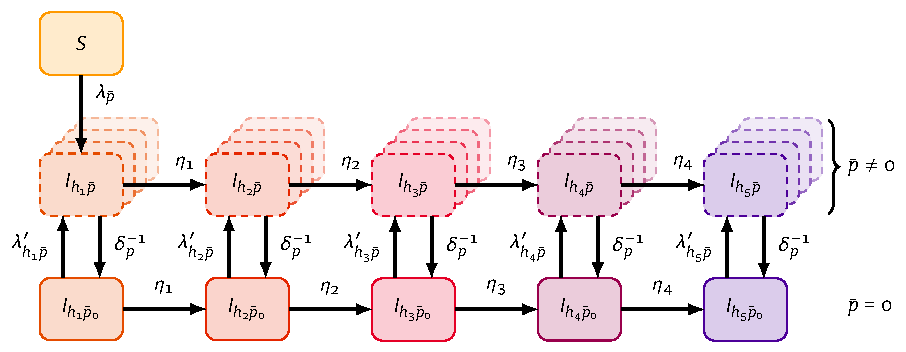
\includegraphics[scale=1]{model.hiv.p}
  \caption{Modelled states and transitions related to HIV infection,
    and a new stratification $\p$ to track
    the proportions of individuals in partnerships where transmission already occurred}
  \label{fig:model.hiv.p}
  \floatfoot{
    $S$: susceptible;
    $I_{h}$: infectious in stage $h$;
    $p$: partnership type;
    $\p$: new stratification, where
      $\p = 0$ reflects no recent transmission (all new partnerships), and
      $\p \ne 0$ reflects recent transmission via a type-$p$ partnership;
    $\lambda$: force of infection per susceptible;
    $\lambda'$: force of infection per infectious;
    $\eta$: rate of progression between infection stages;
    $\delta$: partnership duration.}
\end{figure}
%===================================================================================================
\subsection{Equations%
  \footnote{\shortquote{Enough talk. Show me the \$} --- \LaTeX\ users.}}\label{foi.prop.eq}
Since partnership duration is now considered separately and explicitly,
I do not define any per-partnership probability of transmission $B$.
Rather, I define the force of infection to directly include
the frequency of sex per partnership $F$ and probability of transmission per sex act $\beta$.
However, the mixing is now slightly more complicated,
since the number of ``effective partnerships'' depends on infection status.
In addition, these partnerships are now defined as numbers of concurrent partners $K$,
rather than partnership formation rates $Q$.
\par
Let $M_{pii'}$ be the total (population-level, not per-person)
number of type-$p$ partnerships between group $i$ and group $i'$.
As described \sref{model.par.mix}, this ``mixing matrix'' $M_{pii'}$ can be defined in several ways,
based on the total numbers of ``effective partnerships'' among each group: $M_{pi}, M_{pi'}$,
plus some parameter(s) specifying mixing patterns (\eg $\Phi$).
Working backwards, I start by defining $M_{pi}$ (and likewise $M_{pi'}$) via
the sum across health statuses --- \ie susceptible, and different stages of infection $h$:
\begin{equation}\label{eq:M.SI}
  M_{pi} = M_{S,pi} + \sum_h M_{I,pih}
\end{equation}
I then define the total numbers of partnerships among susceptible individuals as:
\begin{equation}
  M_{S,pi} = S_{i} K_{pi} \label{eq:M.S}
\end{equation}
and likewise for individuals in infection stage $h$:
\begin{equation}
  M_{I,pih} = I_{ih,\p=p} (K_{pi}-1) + \sum\nolimits_{\p \ne p} I_{ih\p}\,K_{pi} \label{eq:M.I}
\end{equation}
\eqref{eq:M.I} is the key equation whereby
the  numbers of ``effective type-$p$ partnerships'' among
individuals in stratum $\p$ are reduced by 1.
This reduction is then propagated through the mixing patterns when defining $M_{pii'}$.
% TODO: (*) double-check that this reduction should be propagated through the mixing patterns
Thus, we are now ready to construct the overall force of infection equation as follows.
I define the total (population-level, not per-person) rate of transmission
from group $i'$ and infection stage $h'$ to group $i$ via type-$p$ partnerships as:
\begin{equation}
  \Lambda_{pii'h'} = F_p \beta_{pii'h'} M_{pii'}
  \left(\frac{M_{S,pi}}{M_{pi}}\right)
  \left(\frac{M_{I,pi'h'}}{M_{pi'}}\right)
\end{equation}
where the two fractions represent the proportions of all partnerships $M_{pii'}$
formed between susceptible individuals from group $i$ ($M_{S,pi}$)
and infectious individuals in group/infection stage $i'h'$ ($M_{I,pi'h'}$).
The per-person transmission rates to group $i$, and from group $i'h'$ can then be defined as:
\begin{alignat}{1}
  \lambda_{pi} &= \sum_{i'h'} \Lambda_{pii'h'}\,{S_{i}}^{-1} \label{eq:foi.i} \\
  \lambda'_{pi'h'} &= \sum_{i} \Lambda_{pii'h'}\,{I_{i'h'}}^{-1} \label{eq:foi.jh}
\end{alignat}
For the purposes of solving the model,
we can skip division by $S_{i}$ and $I_{i'h'}$ in \eqrefs{eq:foi.i}{eq:foi.jh},
since $\lambda'_{pi}$ and $\lambda'_{pi'h'}$ are immediately multiplied by $S_{i}$ and $I_{i'h'}$,
respectively, in the system of differential equations.
\par
Finally, and to reiterate from above, infected individuals in stratum $I_{ih\p}$
are assumed to form new partnerships at a rate $\delta_p^{-1}$,
and thereby transition to stratum $I_{ih\p_0}$ (``all new partners''); and
otherwise transition between infection stages, cascade of care, activity groups, etc. as usual,
as illustrated in Figure~\ref{fig:model.hiv.p}.
%===================================================================================================
\subsection{Transmission via Multiple Partnerships}\label{foi.prop.mp}
In the proposed \emph{Effective Partnerships Adjustment} approach,
I do not explicitly model the proportions of infected individuals
who recently acquired and/or transmitted infection via
two different partnership types, or two partnerships of the same type.
To do so, the required size of the new dimension $\p$ would be at least $2^{P}$, not $P+1$,
where $P$ is the number of different types of partnerships modelled.
For transmission via three different partnerships, the required size would be at least $3^P$, etc.
Indeed, this exponential relationship is related to the challenge of specifying
all possible combinations of partnership states in pair-based models \cite{Kretzschmar2017}.
However, under frequentist assumptions, we can equivalently model
two transmissions by one individual as one transmission each by two individuals.
Thus, we can transfer two individuals from $I_{ih\p_0}$ to
$I_{ih\p_1}$ and $I_{ih\p_2}$ (one each) under the $P+1$ stratification,
instead of just one individual from $I_{ih\p_0}$ to
``$I_{ih\p_{12}}$'' under one of the exponential $x^P$ stratifications.
\par
In fact, $I_{ih\p_0}$ can be \emph{negative} (but only for $\p = 0$),
because the dimension $\p$ is only relevant to \eqref{eq:M.I};
in all other contexts and equations,
we use $I_{ih} = \sum_{\p} I_{ih\p}$, which must be positive as usual.
Moreover, we can also have $I_{ih\p} > I_{ih}$, provided that:
\begin{equation}\label{eq:I.constr}
  I_{ih\p} \le I_{ih} K_{pi}
\end{equation}
reflecting the situation where 100\% of $I_{ih}$
have recently acquired and/or transmitted infection via at least one type-$p$ partnership,
or 50\% via at least two partnerships, etc.
This situation can therefore only arise in the context of
multiple concurrent type-$p$ partnerships: $K_{pi} > 1$.
If $I_{ih\p} > I_{ih}$, then $I_{ih\p_0}$ \emph{must} be negative,
but we can show that \eqref{eq:M.I} still yields the correct value of $M_{I,pih}$.
With this perspective, the constraint in \eqref{eq:I.constr} may be more intuitive:
we cannot ``remove'' more than the total number of partnerships.
This constraint should also be easy to guarantee for a small enough timestep,
because $M_{I,pih}$ approaches zero as $I_{ih\p}$ approaches $I_{ih} K_{pi}$
--- i.e. all type-$p$ partnerships become \hivp seroconcordant,
and no more transmission can occur via these partnerships until partners change.
% TODO: (?) add serosorting refs: cross-sectional vs individual-cohort \cite{Wang2020,Kim2020}
